In this section, the aim is to predict the performance of the speaker, from his characteristics derived from the analysis of testing and training data. If we are able to reliably predict  if the $Spkshow$ will be correctly recognized or not, when analysing the main features contributing to this prediction, we can identify the features that  facilitates or hamper the identification, for a given system.

At each $SpkShow$ is associated the maximal $Fm$ obtained accross systems. Doing so, we do not focus on a particular system, but we try to explain "the-best-we-can-do" performance for each $SpkShow$.
As we have seen in the previous section that the performance is essentially bi-modal (the speaker is not recognized at all vs the speaker is well recognized), we focus on the task of predicting, for a given $SpkShow$, if the $Fmax$ will be equal to zero or not.

Many parameters, resulting from the analysis of the training or the testing data, could be potentially used for this classification task. For instance, parameters related to the linguistic content of the speech turns, the prosody or the ambiant noise could be studied.

We restrict our work, in a first attempt, to the families of parameters derived from the analysis of speech segment distribution for the testing data, and from the training data parameters, because they are straightforward to compute, and easily interpretable.

In the family of parameters based on training data, the potential parameters are derived from the analysis of the amount of  training data available for $SpkShow$ in the system that gives the $Fmax$:
\begin{itemize}
\item total duration of training data
\item total number of training sessions
\item duration of training data from REPERE corpus
\item number of training sessions from REPERE corpus
\item duration of training data from external corpus (non-REPERE)
\item number of training sessions from external corpus
\end{itemize}
With these parameters, we investigate the importance of the variability of the training data (in terms of number of sessions and type of corpus)

In the family of parameters derived from the speech segment distribution of the testing data, the potential parameters, for each $SpkShow$, are:
\begin{itemize}
\item total duration of the speech turns of $SpkShow$
\item average duration of the speech turns of $SpkShow$
\item duration of the longest speech turn of $SkShow$
\item number of speech turns of $SpkShow$
\item total duration of overlapped speech segments of $SpkShow$
\item number of overlapped speech segments of $SpkShow$
\item normalized duration of $SpkShow$ (i.e. total duration of speech turns of $SpkSghow$ divided by the total duration of speech for the whole show)
\item normalized number of speech segments of $SpkShow$ (i.e.   number of speech turns of $SpkShow$ divided by the total number of speech turns for the whole show) 
\item average pause duration preceding the speech turns of $SpkShow$
\item average pause duration following the speech turns of $SpkShow$
\end{itemize}

As far as the classifier is concerned, it is preferable to chose a classifier that enables an easy interpretation of the results and the importance of each parameters, more than a black box, leading to good classifier results, without any interpretation. That's why we choose a classification tree predictor (quelle ref pour le classifier de scikit learn???).
As the corpus is limited (305 $SpkShow$), it was treated in a leave-one-out fashion: for each $SpkShow$, a classification tree is trained on the corpus minus the $SpkShow$, and applied on the parameters of $SpkShow$ to predict if his $Fmax$ will be zero or not. The global performance is thus obtained concatenating the performance obtained for each $SpkShow$ separately.
As the corpus in unbalanced (63 $SpkShow$ with $Fmax=0$, and 242 $SpkShow$ with $Fmax>0$), the performance is not evaluated in terms of classification errors, but in terms of prediction and recall for each class of speakers. Precision and recall rates, and F-measure,  are computed to evaluate the task of detecting $SpkShow$ with $Fmax=0$ and symetrically, precision and recall rates, and F-measure are computed to evaluate the task of detection $Spkshow$ with non-zero $Fmax$

Among all the potential parameters listed before, not everyone is usefull, but some can hamper the performances, due to the training process of the tree. Hence, we apply an optimization heuristic to select the best subset of parameters, among the initial set of potential parameters. It is an iterative process, that starts with the whole set of parameters, and at each iteration, removes the parameters without which the best performances are obtained. It ends when there is no parameter to remove. This process leads to a curve of performance in function of the subset of selected parameters (here restricted to a function of the number of selected parameters), and for analysing the result, we focus on the subset which gives the best classification performance.

 The results of the classification process, in a leave-one-out fashion, for the initial set of parameters, and for the selected subset of parameters are given in table\ref{tableresult}.
\begin{table*}[t]
\begin{center}
\begin{tabular}{r||c|c|c||c|c|c|}
& \multicolumn{3}{c}{all parameters}& \multicolumn{3}{c}{optimal parameters subset}\\\hline
& Prec & Recall & F-measure & Prec & Recall & F-measure \\\hline
Detection of $SpkShow$ with $Fmax=0$ & 75.8 & 79.0 & 77.4 & 80.0 & 82.7 & 81.4 \\\hline
Detection of $SpkShow$ with $Fmax>0$ & 94.5 & 93.4 & 94.0 & 95.6 & 94.6 & 95.0 \\\hline
\end{tabular}
\caption{Detection performance of classifier}
\label{tableresult}
\end{center}
\end{table*}


\subsection{Detection}


\subsection{Prediction}


\begin{figure}[t]
\centering
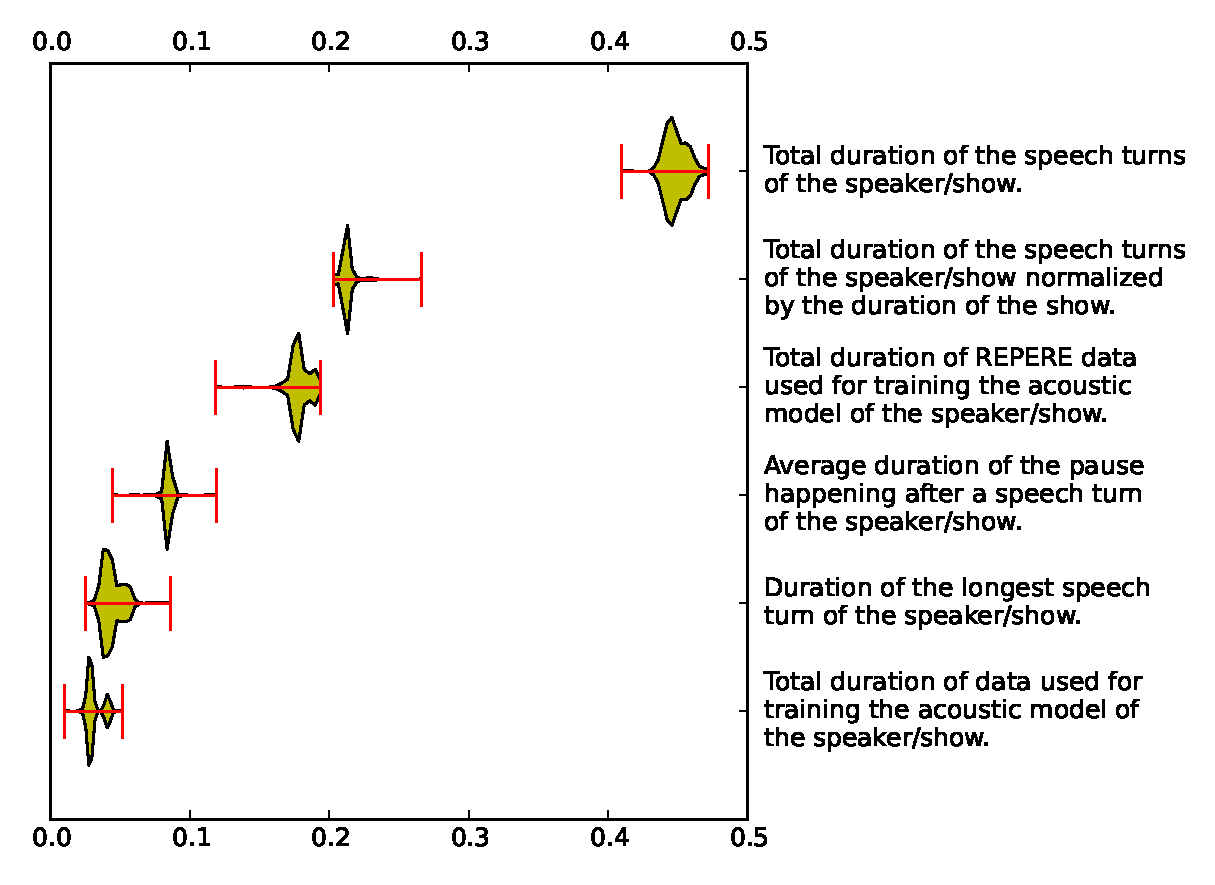
\includegraphics[width=\linewidth]{figures/violin.eps}
\caption{Distribution of feature importance.}
\label{fig:featureImportance}
\end{figure}


Feature importance === Gini coefficent~\cite{Breiman2001}


\begin{figure}[t]
\centering
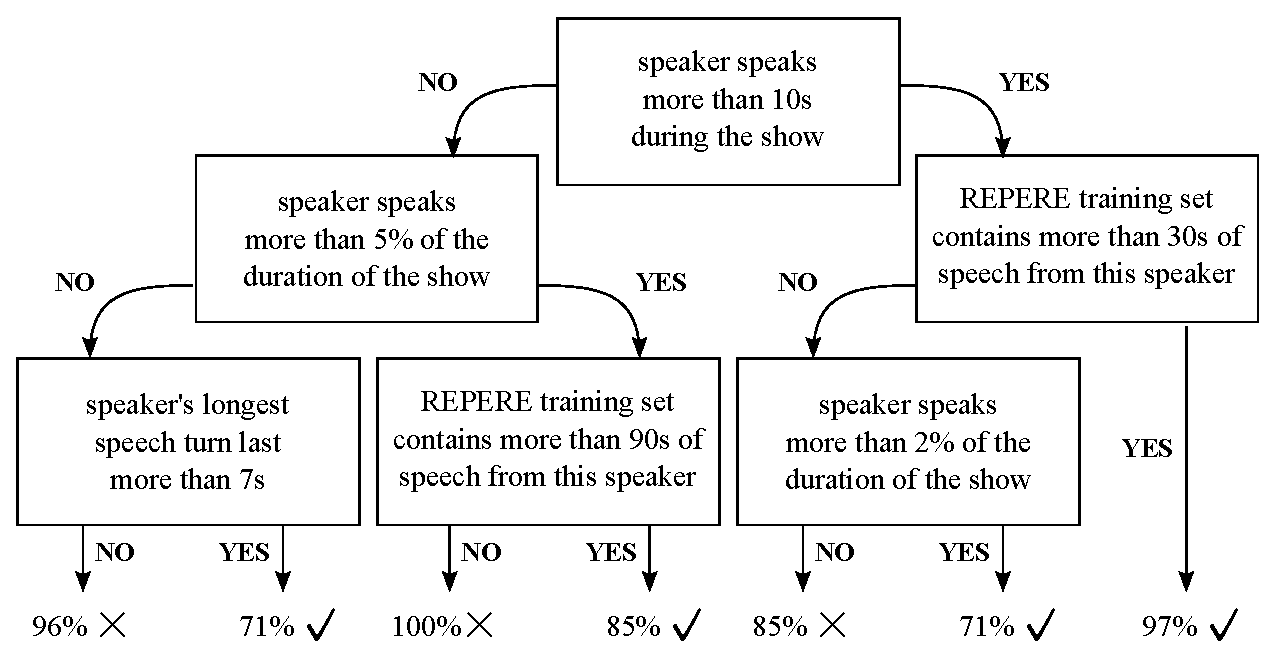
\includegraphics[width=\linewidth]{figures/tree.eps}
\caption{Not recognized ($\times$) vs. (partially) recognized ($\checkmark$)}
\label{fig:tree}
\end{figure}
